\documentclass[12pt]{article}
\usepackage{amsmath,amsfonts,amsthm,amssymb,wasysym}
\usepackage{setspace}
\usepackage{enumitem}
\usepackage{Tabbing}
\usepackage{fancyhdr}
\usepackage{lastpage}
\usepackage{chngpage}
\usepackage{url}
\usepackage{subfigure}
\usepackage{array}
\usepackage{multicol}
\usepackage[color=blue!40]{todonotes}
\usepackage[protrusion=true,expansion,kerning]{microtype}
\usepackage{natbib}

% to adjust margins:
\topmargin=-0.25in
\evensidemargin=0in
\oddsidemargin=0in
\textwidth=6.25in
\textheight=8.5in
\headsep=0.25in

% homework specific information
\newcommand{\hmwkTitle}{CS791AN Final Project}
\newcommand{\hmwkDueDate}{December 13, 2013}
\newcommand{\hmwkClass}{}
\newcommand{\hmwkClassInstructor}{}
\newcommand{\hmwkAuthorName}{Emma Strubell \\ Jesse Lingeman}

% header and footer
\pagestyle{fancy}
\lhead{\hmwkAuthorName}
\chead{\hmwkTitle}
\rhead{\hmwkDueDate}   
\lfoot{}
\cfoot{}
\rfoot{\emph{Page\ \thepage\ of\ \pageref{LastPage}}}                          
\renewcommand\headrulewidth{0.4pt}
\renewcommand\footrulewidth{0.4pt}

\makeatletter
\newenvironment{tablehere}
  {\def\@captype{table}}
  {}

\newenvironment{figurehere}
  {\def\@captype{figure}}
  {}
\makeatother

%\renewcommand{\bibsection}{\subsubsection*{\refname}}

% Make title 
\title{
\LARGE\bf Low-level NLP Error Analysis \\
\date{}
\author{ Jesse Lingeman \and Emma Strubell}
}

\begin{document}

\maketitle

\begin{abstract}
We perform some basic error analysis on three low-level NLP tasks as implemented in FACTORIE: part-of-speech tagging, dependency parsing, and named entity regognition.
\end{abstract}

\thispagestyle{fancy}

%\begin{multicols}{2}

\section{Introduction}
Error analysis is important to any model, and may potentially reveal important aspects about where the algorithm is failing during a given application. This is especially important in pipelines, where errors created early on in the system will propagate forwards throughout the system, causing upstream errors that may not be easily diagnosable at such a high level. In this work, we take a look at the low-level pipeline errors in Factorie, and propose some potential fixes in order to prevent these errors from flowing to algorithms further downstream.

We will analyze the errors of the Part-Of-Speech (POS), Named Entity Recognition (NER), and Dependency Parsing algorithms available in Factorie \citep{mccallum09:factorie:}, and propose several potential fixes to help reduce these errors. The main goal is to identify where these algorithms are failing, and to fix them at early stages before these errors are masked by down-steam analysis.

\section{Data}
We will be using separate datasets to analyze Factorie’s algorithms. CoNLL2003 ***citation*** is used to benchmark the performance of the POS tagger and the NER tagger, while Ontonotes ***citation*** is used to benchmark the performance of the dependency parser. The POS tagger in Factorie is trained on the Ontonotes data, but is used to analyze the CoNLL2003 data. This is done to simulate a real-world example where we may be running a POS tagger on a dataset we are unable to train on due to data size limitations.

\section{Methods}
Experiments were run using the NLP software package Factorie. The pre-trained Factorie-included POS and NER taggers were used for the tagging experiments, and the standard Factorie dependency parser with modified hyperparameters (shown in Table ***) was used to create dependency trees for each sentence.

The CoNLL2003 and Ontonotes datasets come pre-tokenized, and this tokenization was used in the experiments. These data also include the hand-annotated POS, NER, and parse tags for each token in the document. The inferred tags from each of the algorithms were compared against the hand-annotated tags for correctness. Our error analyses were performed using Python and the SciPy package ***citation***.

\section{Discussion}
Detailed error analysis is important for understanding when and where a particular algorithm is failing to correctly infer data. Moving beyond the F1-score and delving deep into particular errors an algorithm makes can illuminate interesting artifacts about the data, the algorithm, and their interaction. For example, we may find that an algorithm is consistently failing at a particular tag, and it would be easy to correct this deficiency by either adding a new feature or term to the model, or by simply correcting it in post-processing.

\subsection{Part-of-speech tagger errors}
The POS tagger was run on Test A of the CoNLL2003 dataset. A confusion matrix of the inferred tags with the gold tags is shown in Figure ***. The most common error that the Factorie POS tagger made was tagging the word “to” as “IN”, instead of the special tag “TO”. This occurred 332 times in the dataset, accounting for a 0.6% drop in accuracy. This particular error is easily fixed by simply forcing the word “to” to have the tag “TO”. Fixes of this type can occur either in the model itself by attempting to add features or rules that will force the model to do this, or by simply modifying the model’s output in post-processing.
The second type of error is more difficult to unravel. In 308 instances, the POS tagger incorrectly guessed that a noun (“NN”) was a proper noun (“NNP”). However, examination of these incorrect guesses points to some possible issues with the gold-standard tagging of the data. Consider the following two neighboring sentences in the CoNLL2003 corpus:

********PUT ME IN A BOX*********
1. “Essex, however, look certain to regain their top spot after Nasser Hussain and Peter Such gave them a firm grip on their match against Yorkshire at Headingley.”
2. “Hussain, considered surplus to England’s one-day requirements, struck 158, his first championship century of the season, as Essex reached 372 and took a first innings lead of 82.”
********END PUT ME IN A BOX*********

In sentence 1 “Hussain” is correctly tagged as a proper noun (“NNP”), but in sentence 2 “Hussain” is tagged as a noun (“NN”). This is obviously incorrect, as “Hussain” in sentence 2 is referring to the person Nasser Hussain referenced in sentence 1. Even more alarmingly, in sentence 1, “Peter Such” has the labels “NNP” for “Peter”, which is correct, but then verb (“JJ”) for “Such”, which is incorrect because it is a surname. These types of errors with the tags given with the document are quite alarming, and may indicate that they may not be the best comparison to use.

However, the third most common type of error is another simple one to fix. The Factorie POS tagger is using the tag “``” to indicate the opening of quotes. The CoNLL2003 dataset does not differentiate between opening and closing quotes with their tags, so forcing all inferred opening tags to be the normal quote tag will also improve the overall accuracy.

\subsection{Named-entity recognition errors}
For the NER task we used Factorie’s built-in NER tagger, which was trained on the CoNLL2003 dataset. We again used the Test A document of CoNLL2003. The confusion matrix of the different error types is shown in Figure ***. Overall, the Factorie NER tagger performed very well, achieving 98\% accuracy on the dataset. By looking at the errors, we can see that the most common type of error is when the NER algorithm infers the tag “O” for what should be a named entity. The most common case of this is “U-MISC”, which makes sense intuitively as miscellaneous entities probably look the most like other nouns. This error happened 65 times. Exploring the data, we find that many of the errors involve hyphenated words, such as “ex-England”, “post-Games”, and “ex-Milan”. 

The second most common error is labeling a token as “O” instead of “U-ORG”, which occurred 49 times. This seems a little more surprising, surely it should be relatively easy to tell the difference between a non-named entity and an organization? When we take a look at the data, it a clear pattern emerges. Most of the errors include tokens such as “FOMC”, “SDA”, and “DNIB”. So it may not be very good at guessing the acronym form of an organization. Mixed in are errors where the organization name may be a different word in its own context, such as “Real” or “Fed”. It seems like there could be a fairly clear improvement by adding in a feature for non-dictionary all-capitalized words in order to capture these stock acronyms.

\subsection{Parser errors}
Dependency label mistakes made by the parser are depicted as a confusion matrix in Figure \ref{parseconfusion}. The most common dependency labeling mistake was labeling edges that should have been labeled negations as adverbial modifiers. The mistake makes sense since negations make up a subset of adverbial modifiers, but the parser does not appear to ever be assigning the ``neg’’ label. It seems like these mistakes could thus easily be fixed via some simple bug fix or modification to the parser. 

\begin{center}
\begin{figure}[!ht]
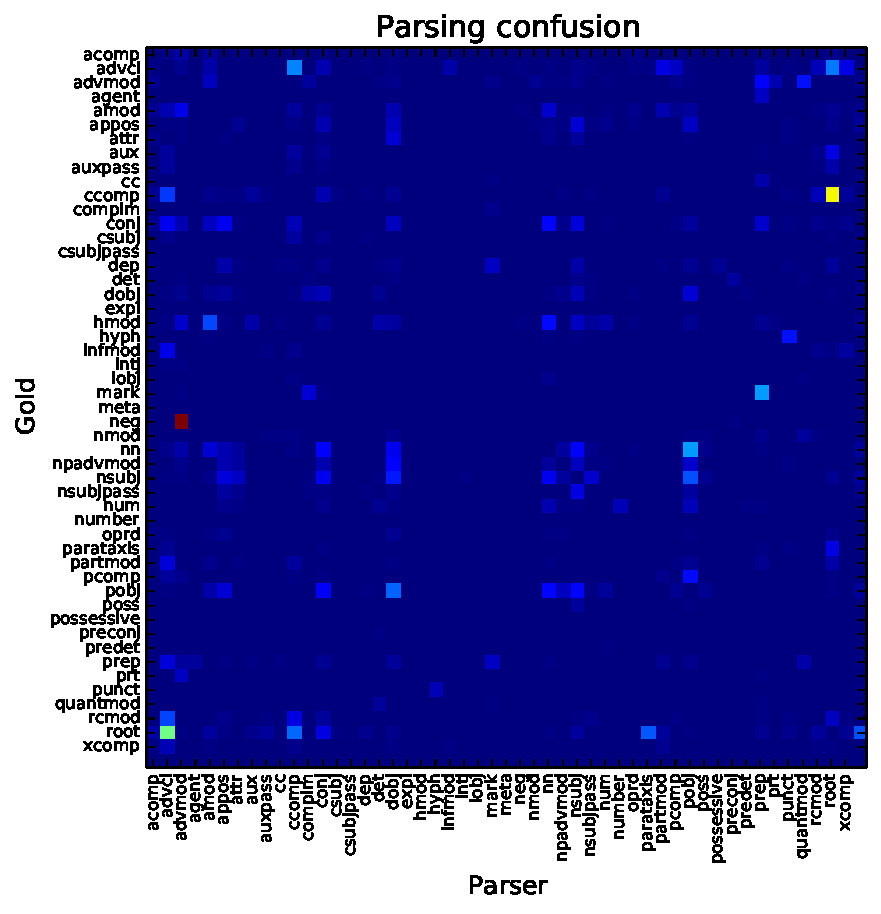
\includegraphics[scale=1.0]{parse_output.pdf}
\caption{Confusion matrix depicting dependency labeling mistakes made by our parser as compared to gold tags \label{parseconfusion}}
\end{figure}
\end{center}

Aside from this fluke, the most frequent parsing errors that we observed seemed to involve (1) subordinate clauses, (e.g. mistaking the root for complementary or adverbial clauses or mistaking them for each other), (2) prepositional phrases, (e.g. confusing prepositional objects with direct objects) and (3) punctuation. Differentiating between these types of syntactic dependencies is known to be difficult, not only for computers but for humans as well. Punctuation is generally ignored in parser accuracy measurements and so we did not analyze parsing errors involving punctuation, but we did observe that many parsing errors were made on punctuation tokens.

Disturbingly, aside from ``neg,’’ the majority of parsing errors involved mislabeling the root; our parser erroneously labeled the root in about 15\% of all the sentences we tested, and the two most frequent labeling errors after ``neg’’ were mistaking the root for an adverbial clause, and labeling the head of complementary clauses as the root. The prevalence of root labeling mistakes is particularly alarming since root errors can easily propagate throughout the entirety of the parse tree, such as in Figure ***\ref{propfig}***. 

The root labeling errors always seemed to occur towards the beginning of the sentence. Further, it appears as though the parser tends to label the first verb in the sentence as the root. This behavior is likely due to the greedy transition-based algorithm that our parser uses to assign dependency labels. In general, we suspect that the prevalence of root mislabeling is very much a product of the greedy algorithm, since many more shift-reduce operations are necessary in the transition-based parser to decide a root label than a simpler modifier leaf in the tree, leaving much more room for mistakes when deciding the root. Due to the inevitable propagation of mistakes from higher-level tokens in the parse tree to lower ones, this is an unfortunate issue with dependency parsing that certainly deserves further analysis into how this aspect of transition-based parsing could be improved. It has been found that adding richer, higher-order features of the tree, such as valency, grand-head and siblings of the current token, can reduce the prevalence of these problems while maintaining the asymptotic speed advantages of transition-based dependency parsing over graph-based algorithms \cite{zhang-nivre-12}. We have added these features to the parser and await the results.

\subsection{Using POS tags to help NER}
When exploring NER errors, it was often observed that when NER incorrectly labeled a token as “O”, the POS tag for that same token was “NNP”. We hypothesized that it would be advantageous to allow the NER tagger to use this information to let it know that it should make a guess when the POS tag indicates it is a proper noun. We tried several different approaches. The first approach we tried was to simply take the highest pre-Viterbi score for the token we the POS tag was inferred to be “NNP” and the NER tagger inferred “O”. However, this naive approach severely hurt the accuracy, as that value was almost never correct. Next, we tried using the second-most-likely Viterbi path, which also turned out to not work.

We then decided to add the POS tag as a feature to the model. The POS tagger was first run on the dataset, and then the inferred POS tag was used as a feature for each token when training for NER. The hyperparameters for the model were the same used for the stock NER model in Factorie. Testing was again done on the CoNLL2003 Test A dataset, and training done on the CoNLL2003 training dataset. Including the inferred POS tag did not help the model: the F1-score dropped from the baseline score of 0.9303 to 0.9300. However, due to the large discrepancies between the Factorie POS tagger and the tags in the dataset, we also retrained using the gold POS tags from the CoNLL2003 dataset. Doing this improved the F1-score of the NER tagger from 0.9303 to 0.9336. We also tested this modification on the more difficult CoNLL2003 Test B dataset, but the F1-score dropped from 0.887 to 0.883, so the utility of this change is unclear. A better approach may be to use an indicator variable of “NNP”/”Not NNP” instead of the raw POS tag itself.

\section{Conclusion}
Error analysis is an extremely important step in understanding the components of a natural language processing pipeline, but that seems less thoroughly studied than it should be. Certainly we know that error propagation is a significant problem in NLP pipelines, and such detailed analysis can reveal where errors are occuring, why they are happening, and how they might be fixed. Indeed, we discovered a number of simple errors involving tag disagreement between training and testing data that could be easily fixed to significantly improve accuracy measurements. Unfortunately, we also discovered mistakes in the labeled data, which is a more difficult problem to address. In the future, we hope to take a more detailed look at the interactions between errors along a more complex pipeline, analyzing how errors in an earlier component influence the errors further down the pipeline. Even the simple, low-level, single-task analysis presented here, though, was revealing, and should be a basic step in any NLP research project.

\bibliography{final_report}
\bibliographystyle{unsrt}

%\end{multicols}

\end{document}

%%% Local Variables: 
%%% mode: latex
%%% TeX-master: t
%%% End: 
